\documentclass[12pt]{article}
\usepackage[a4paper, total={6in, 8in}]{geometry}
\usepackage{amsfonts}
\usepackage{amsmath,amssymb,trimclip,adjustbox}
\usepackage{breqn}
\usepackage{pgfplots}
\usepackage{hyperref}
\usepackage{tabularray}
\usepackage{polski}
\usepackage[utf8]{inputenc}

\setlength{\parindent}{0pt}
\setlength{\textheight}{650pt}
\setlength{\oddsidemargin}{0pt}
\setlength{\textwidth}{480pt}

\hypersetup{
    colorlinks=true,
    linkcolor=blue,
    filecolor=magenta,      
    urlcolor=cyan,
    pdftitle={Overleaf Example},
    pdfpagemode=FullScreen,
}

\author{Michał Puchyr}
\title{Sprawozdanie 100B}

\begin{document}
\maketitle

\section{Cel ćwiczenia}

\begin{itemize}
    \item Pomiar rezystancji na opornikach oraz żarówce
    \item Zmierzenie wartości napięcia i natężenia na opornikach oraz żarówce
    \item Obliczenie oporu przy pomocy praw fizyki i porównanie go z wcześniejszymi pomiarami
    \item Zrozumienie praw fizyki związanych z prądem elektrycznym
\end{itemize}

\section{Opis ćwiczenia}
\subsection{Wstęp teoretyczny}

W obwodach prądu stałego rezystancja jest wielkością charakteryzującą relację między napięciem
a natężeniem prądu elektrycznego. Oznacza to, że opór przewodnika elektrycznego jest 
wprost proporcjonalny do napięcia i odwrotnie proporcjonalny do natężenia.

\label{ohm}
$$ R = \frac{U}{I} $$ 
Gdzie :

$R$ - rezystancja [$\Omega$]

$U$ - napięcie między końcami przewodnika [$V$]

$I$ - natężenie prądu elektrycznego[$A$]\\

Przyrządy i materiały wykorzystane do pomiarów : 
\begin{itemize}
    \item 2 mierniki uniwersalne M8906
    \item Zasilacz stabilizowany
    \item Przewody elektryczne
    \item Zestaw oporników z żarówką
\end{itemize}

\pagebreak Schemat układu nr 1 \\

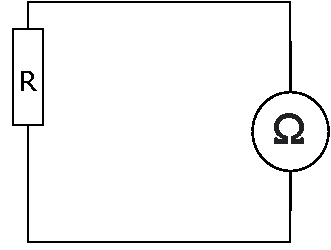
\includegraphics{obwod1.pdf}

Schemat układu nr 2

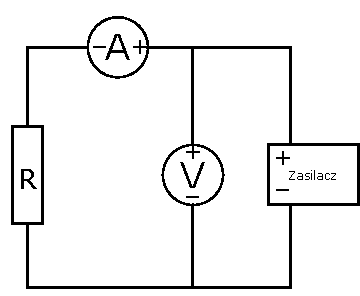
\includegraphics{obwod2.pdf}

\section{Pomiary układów}

\begin{tabular}{ |p{0.5cm}|p{2cm}|p{3cm}|p{3cm}|p{3cm}| }
    \hline
    \multicolumn{5}{|c|}{Pomiary oporu w układzie pierwszym} \\
    \hline
    Lp. &Opornik& Opór [$\Omega$] & Zakres[$\Omega$] & Niepewność[$\Omega$] \\ 
    \hline
    1 & $R_1$ & 165,2 & 200 & 1,62 \\
    2 && 165,3 & 200 & 1,62 \\
    3 && 164,9 & 200 & 1,62 \\
    4 && 165,0 & 200 & 1,62 \\
    \hline
    5& $R_2$ & 122,6 & 200 & 1,28\\
    6&& 122,9 & 200 & 1,28 \\
    7&& 123,0 & 200 & 1,28 \\
    8&& 122,9 & 200 & 1,28 \\
    \hline
    9& Żarówka & 13,9 & 200 & 0,41 \\
    10&& 13,8 & 200 & 0,41\\
    11&& 13,9 & 200 & 0,41\\
    12&& 13,9 & 200 & 0,41\\
    \hline
\end{tabular}

\begin{adjustbox}{center}
\begin{tabular}{|p{0.5cm}|p{1.5cm}|p{1cm}|p{1.5cm}|p{1.5cm}|p{2cm}|p{1.3cm}|p{1.2cm}|p{1.5cm}|p{1.5cm}|}
    
    \hline
    \multicolumn{10}{|c|}{Pomiary napięcia i natężenia w układzie drugim} \\
    \hline
    Lp. & Opornik& U[$V$]& u(U)[V] & I[$10^{-3}A$] & u(I)[$10^{-3}A$] & R[$\Omega$] & $U_c[\Omega]$ & R śr.[$\Omega$] & u($\overline{R}$)[$\Omega$] \\ 
    \hline
    1 & $R_1$ & 3,21 & 0,02 & 19,5 & 0,20 & 164,62 & 1,88 & 163,92 & 0,09\\
    2 && 4,66 & 0,02 & 28,4 & 0,26 & 164,08& 1,66 && \\
    3 && 6,19 & 0,02& 37,7 & 0,32 & 164,19& 1,53 && \\
    4 && 7,70 & 0,03& 47,0 & 0,39 & 163,83& 1,49 && \\
    5 && 9,34 & 0,03& 57,1 & 0,46 & 163,57& 1,44&& \\
    6 && 6,19 & 0,02& 37,8 & 0,32 & 163,76& 1,52&& \\
    7 && 4,65 & 0,02& 28,4 & 0,26 & 163,73& 1,66&& \\
    8 && 3,21 & 0,02& 19,6 & 0,20 & 163,78& 1,86&& \\
    9 && 7,70 & 0,03& 47,0 & 0,39 & 163,83& 1,49&& \\
    10 && 9,34 & 0,03 & 57,0 & 0,46 & 163,86& 1,44&& \\
    \hline
    11 & $R_2$ & 3,20 & 0,02 & 26,2 & 0,24 & 122,14 & 1,27 & 122,05 & 0,05 \\
    12 && 4,63 & 0,02 & 37,9 & 0,33 & 122,16& 1,19 && \\
    13 && 6,16 & 0,02 & 50,4 & 0,41 & 122,22& 1,10 && \\
    14 && 7,66 & 0,03 & 62,8 & 0,50 & 121,97& 1,07 && \\
    15 && 9,29 & 0,03 & 76,2 & 0,59 & 121,92& 1,04 && \\
    16 && 3,19 & 0,02 & 26,2 & 0,24 & 121,76& 1,25 && \\
    17 && 4,63 & 0,02 & 37,9 & 0,33 & 122,16& 1,19 && \\
    18 && 6,16 & 0,02 & 50,4 & 0,41 & 122,22& 1,10 && \\
    19 && 7,65 & 0,03 & 62,7 & 0,50 & 122,01& 1,07 && \\
    20 && 9,29 & 0,03 & 76,2 & 0,59 & 121,92& 1,04 && \\
    \hline
    21 & Żarówka & 3,16 & 0,02 & 43,5 & 0,36 & 72,64 & 0,69 & 93,84 & 4,68 \\
    22 && 4,60 & 0,02 & 54,4 & 0,44 & 84,56& 0,78  && \\
    23 && 6,13 & 0,02 & 63,7 & 0,50 & 96,23& 0,84  && \\
    24 && 7,64 & 0,03 & 73,0 & 0,57 & 104,66& 0,90  && \\
    25 && 9,28 & 0,03 & 82,7 & 0,64 & 112,21& 0,96  && \\
    26 && 3,16 & 0,02 & 43,5 & 0,36 & 72,64& 0,69   &&\\
    27 && 4,60 & 0,02 & 54,4 & 0,44 & 84,56& 0,78   &&\\
    28 && 6,13 & 0,02 & 64,6 & 0,51 & 94,89& 0,84  && \\
    29 && 7,64 & 0,03 & 73,7 & 0,57 & 103,66& 0,89  && \\
    30 && 9,28 & 0,03 & 82,6 & 0,64 & 112,35& 0,96 && \\
    \hline
\end{tabular}
\end{adjustbox}\\

Rezystancja w układzie drugim została obliczona przy użyciu \hyperlink{ohm}{prawa Ohma}.
Pomiary zostały wykonane przy zakresie 200mA i 20V.

\subsection{Wykres I = f(U)}

\subsubsection{Wykres dla pomiaru opornika R1}
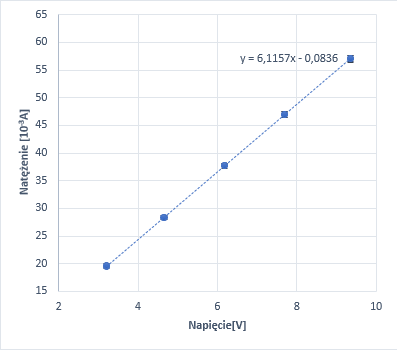
\includegraphics{pomiar1.png}

\subsubsection{Wykres dla pomiaru opornika R2}
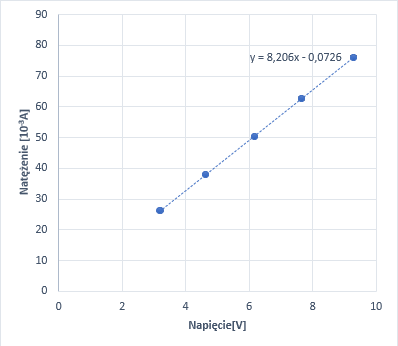
\includegraphics{pomiar2.png}

\subsubsection{Wykres dla pomiaru żarówki}
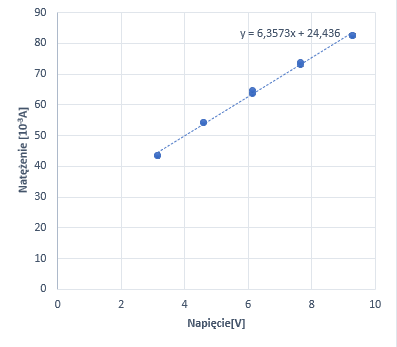
\includegraphics{pomiar3.png}

\section{Obliczenia}
\subsection{Niepewność typu A}

Do obliczenia niepewności pommiarowej typu A został wykorzystany poniższy wzór

$$ u_a(x) = \sqrt{\frac{\sum\limits_{i=1}^{n}(x_i - \overline{x})^2}{n(n - 1)}} $$
$$ \overline{x} = \frac{1}{n}\sum\limits_{i = 1}^{n}x_i $$

Dla pierwszego opornika : 

$ \overline{x} = 163,92\Omega $

$ u_a(x) = 0,09\Omega $\\

Dla drugiego opornika : 

$ \overline{x} = 122,05\Omega $

$ u_a(x) = 0,05\Omega $\\

Dla żarówki : 

$ \overline{x} = 93,84\Omega $

$ u_a(x) = 4,68\Omega $

\subsection{Niepewność typu B}

Do obliczenia niepewności pomiaru napięcia (zakres 20V) przez miernik wykorzystano wzór
$$ \pm 0.5\% rdg + 1dgt  $$
Do obliczenia niepewności pomiaru natężenia (zakres 200mA) przez miernik wykorzystano wzór
$$ \pm 1.2\% rdg + 1dgt  $$
Do obliczenia niepewności pomiaru oporu (zakres 200$\Omega$) przez miernik wykorzystano wzór
$$ \pm 0.8\% rdg + 3dgt  $$

\subsection{Niepewność typu C}

Do obliczenia tej niepewności dla danego pomiaru wykorzystano wzór

$$ u_c(x) = \sqrt{(\frac{\partial f}{\partial U})^2 u(U)^2 + (\frac{\partial f}{\partial I})^2 u(I)^2 } $$

$$ u_c(x) = \sqrt{(\frac{1}{I})^2 u(U)^2 + (\frac{-U}{I^2})^2 u(I)^2 } $$

\section{Wnioski}
Poprzez wykonanie pomiarów natężenia i napięcia w układach można zauważyć, że napięcie i natężenie
w opornikach
zwiększają się proporcjonalnie względem siebie co wynika z \hyperlink{ohm}{prawa Ohma}. Poprzez
pomiar pierwszy i porównanie wyników pomiaru drugiego można zaobserwować identyczność (z małymi
odchyleniami) zmierzonego oporu z tym obliczonym przy pomocy wzoru. \\
Żarówka ze względu na zmienność temperatury nie zastosowuje się do prawa Ohma, opór zmieniał się 
w zależności od wielkości napięcia i natężenia nieliniowo. Opór zmierzony na żarówce jest znacząco
różniący się od tego, wyliczonego przy pomocy \hyperlink{ohm}{prawa Ohma}.

\section{Bibliografia}
\begin{itemize}
    \item \url{https://pl.wikipedia.org/wiki/Prawo_Ohma}
\end{itemize}

\end{document}